\documentclass[a4paper]{article}
%\usepackage[utf8]{inputenc}
\usepackage[spanish, es-tabla, es-noshorthands]{babel}
\usepackage[table,xcdraw,dvipsnames]{xcolor}
\usepackage[a4paper, footnotesep=1.25cm, headheight=1.25cm, top=2.54cm, left=2.54cm,
 bottom=2.54cm, right=2.54cm]{geometry}
%\geometry{showframe}
 \usepackage[normalem]{ulem}
 \useunder{\uline}{\ul}{}

%VERIFICAR EL HEAD Y EL FOOT EN
%https://ctan.dcc.uchile.cl/macros/latex/contrib/geometry/geometry.pdf

%Paquetes varios:
\usepackage{verbatimbox}

%\usepackage{wrapfig}			%Wrap figure in text
\usepackage[export]{adjustbox}	%Move images
\usepackage{changepage}			%Move tables
\usepackage{todonotes}

\usepackage{tikz}
\usepackage{amsmath}
\usepackage{amsfonts}
\usepackage{amssymb}
\usepackage{float}
\usepackage[graphicx]{realboxes}
\usepackage{caption}
\usepackage{subcaption}
\usepackage{multicol}
\usepackage{multirow}
\setlength{\doublerulesep}{\arrayrulewidth}
%\usepackage{booktabs}

\usepackage{array}
\newcolumntype{C}[1]{>{\centering\let\newline\\\arraybackslash\hspace{0pt}}m{#1}}
%\usepackage[american]{circuitikz}
\usetikzlibrary{calc}
\usepackage{fancyhdr}
\usepackage{units} 

\usepackage{colortbl}
%\usepackage{sectsty}
%\usepackage{unicode-math}

%FONTS (IMPORTANTE): Compilar en XeLaTex o LuaLaTeX
\usepackage{anyfontsize}	%Font size
\usepackage{fontspec}		%Font type
%Si sigue sin andar comentar \usepackage[utf8]{inputenc}
%https://ctan.dcc.uchile.cl/macros/unicodetex/latex/fontspec/fontspec.pdf
%https://www.overleaf.com/learn/latex/XeLaTeX

%Path para imagenes para trabajar en subarchivos
\graphicspath{{../Resumen/}{../Referencias/}{../Apendice/}{../Descripción de la Empresa/}{../Tareas del Alumno/}{../Conclusiones/}{../Herramientas Empleadas/}}

%Definiciones de nuevos comandos y colores
%COLORES:
\definecolor{AzulFoot}{rgb}{0.682,0.809,0.926}	%RGB	%{174,206,235}
\definecolor{AzulInfo}{rgb}{0.180,0.455,0.710}	%RGB	%{46,116,181}
\definecolor{AzulTable}{rgb}{0.302,0.507,0.871}	%RGB	%{68,114,196}
\definecolor{PName}{rgb}{0.353,0.353,0.353}		%RGB	%{90,90,90}
\definecolor{mygreen}{rgb}{28,172,0} % color values Red, Green, Blue
\definecolor{mylilas}{rgb}{170,55,241}

%Change Font Size

% #1 = size, #2 = text
\newcommand{\setparagraphsize}[2]{{\fontsize{#1}{6}\selectfont#2 \par}}		%Cambia el size de todo el parrafo
\newcommand{\setlinesize}[2]{{\fontsize{#1}{6}\selectfont#2}}				%Cambia el font de una oración

%IMAGE IN TABLE:			%Ejemplo: \includeintable{.3}{ImagenesFactibilidad/pend}
\renewcommand\fbox{\fcolorbox{white}{white}}
\setlength{\fboxrule}{0pt}	%padding thickness
\setlength{\fboxsep}{4pt}	%border thickness
\newcommand{\includeintable}[2]{	
	\fbox{
		\begin{minipage}{#1\textwidth}
        	\includegraphics[width=\linewidth]{#2}
    	\end{minipage}
	}
}

%LINK IN REF
\newcommand{\reflink}[1]{		%LINK
	\href{#1}{#1}
}

%NOTAS:
\newcommand{\note}[1]{		%RED BIG NOTE (TODO)
	\begin{center}
		\huge{ \textcolor{red}{#1} }
	\end{center}
}

\newcommand{\lnote}[1]{{\fontsize{14}{6}\selectfont\textcolor{green}{#1}}}	%Notas pequeñas

\newcommand{\observacion}[2]{  \ifnumequal{1}{#1}{ { \todo[inline,backgroundcolor=red!25,bordercolor=red!100]{\textbf{Observación: #2}} } }{  }  }

\newcommand{\red}[1]{\textcolor{red}{#1}}

\newcommand{\TBD}{\textcolor{red}{(TBD) }}
\newcommand{\tbd}{\textcolor{red}{(TBD) }}

\newcommand{\TBC}{\textcolor{red}{(TBC) }}
\newcommand{\tbc}{\textcolor{red}{(TBC) }}

\newcommand{\quotes}[1]{``#1''}
\newcommand{\q}[1]{``#1''}

\newcommand{\ip}{192.168.0.10:1880}
\newcommand{\ipadmin}{192.168.0.10:1880/admin}

% Comandos para agregar elementos en tablas de acronimos y definiciones
\newcommand{\addacronym}[2]{\textbf{#1} & \begin{tabular}[l]{@{}l@{}}#2\end{tabular} \\ \hline}

% tabItem
\newcommand{\tabitem}{~~\llap{\textbullet}~~}


\usepackage{hyperref}
\hypersetup{
    colorlinks=true,
    linkcolor=black,
    filecolor=magenta,      
    urlcolor=AzulInfo,
    citecolor=AzulInfo,    
}

%Configuración del header y del footer:
\usepackage{etoolbox}
\pagestyle{fancy}
\fancyhf{}
\rfoot{\thepage}
\renewcommand{\footrulewidth}{4pt}
\renewcommand{\headrulewidth}{0pt}
\patchcmd{\footrule}{\hrule}{\color{AzulFoot}\hrule}{}{}

%Código en el informe
%% IMPORTANTE:
% Verificar que esté \usepackage[dvipsnames]{xcolor}

%\usepackage{listingsutf8}
\usepackage{listings}

\renewcommand{\lstlistingname}{Código}

%LSTSET: Pone un recuadro y contador de linea en el codigo
\newcommand{\boxstyle}{
	\lstset{
		basicstyle=\sffamily\color{black},
		frame=single,
		numbers=left,
		numbersep=5pt,
		numberstyle=\color{gray},
		showspaces=false,
		showstringspaces=false
	}
}

\newcommand{\defaultstyle}{
	\lstset{
		basicstyle=\sffamily\color{white},
		frame=none,
		numbers=none,
		showspaces=true,
		showstringspaces=true
	}
}

\lstdefinelanguage{Kotlin}{
  captionpos=b,
  comment=[l]{//},
  commentstyle={\color{gray}\ttfamily},
  emph={filter, first, firstOrNull, forEach, lazy, map, mapNotNull, println},
  emphstyle={\color{OrangeRed}},
  identifierstyle=\color{black},
  keywords={!in, !is, abstract, actual, annotation, as, as?, break, by, catch, class, companion, const, constructor, continue, crossinline, data, delegate, do, dynamic, else, enum, expect, external, false, field, file, final, finally, for, fun, get, if, import, in, infix, init, inline, inner, interface, internal, is, lateinit, noinline, null, object, open, operator, out, override, package, param, private, property, protected, public, receiveris, reified, return, return@, sealed, set, setparam, super, suspend, tailrec, this, throw, true, try, typealias, typeof, val, var, vararg, when, where, while},
  keywordstyle={\color{NavyBlue}\bfseries},
  morecomment=[s]{/*}{*/},
  morestring=[b]",
  morestring=[s]{"""*}{*"""},
  ndkeywords={@Deprecated, @JvmField, @JvmName, @JvmOverloads, @JvmStatic, @JvmSynthetic, Array, Byte, Double, Float, Int, Integer, Iterable, Long, Runnable, Short, String, Any, Unit, Nothing},
  ndkeywordstyle={\color{BurntOrange}\bfseries},
  sensitive=true,
  stringstyle={\color{ForestGreen}\ttfamily},
}

\lstdefinelanguage{Swift}
{
  morekeywords={
    open,catch,@escaping,nil,throws,func,if,then,else,for,in,while,do,switch,case,default,where,break,continue,fallthrough,return,
    typealias,struct,class,enum,protocol,var,func,let,get,set,willSet,didSet,inout,init,deinit,extension,
    subscript,prefix,operator,infix,postfix,precedence,associativity,left,right,none,convenience,dynamic,
    final,lazy,mutating,nonmutating,optional,override,required,static,unowned,safe,weak,internal,
    private,public,is,as,self,unsafe,dynamicType,true,false,nil,Type,Protocol,
  },
  morecomment=[l]{//}, % l is for line comment
  morecomment=[s]{/*}{*/}, % s is for start and end delimiter
  morestring=[b]", % defines that strings are enclosed in double quotes
  breaklines=true,
  escapeinside={\%*}{*)},
  numbers=left,
  captionpos=b,
  breakatwhitespace=true,
  basicstyle=\linespread{1.0}\ttfamily, % https://tex.stackexchange.com/a/102728/129441
}

\definecolor{keyword}{HTML}{BA2CA3}
\definecolor{string}{HTML}{D12F1B}
\definecolor{comment}{HTML}{008400}

\newcommand{\swiftstyle}{
	\lstset{
  		language=Swift,
  		inputencoding=utf8x,
		extendedchars=\true,
	  	basicstyle=\ttfamily,
	  	showstringspaces=false, % lets spaces in strings appear as real spaces
  		columns=fixed,
  		keepspaces=true,
  		keywordstyle=\color{keyword},
  		stringstyle=\color{string},
  		commentstyle=\color{comment}
	}
}


%Como usarlo:

%\begin{lstlisting}[caption={Simple code listing.}, label={lst:example1}, language=Kotlin]
%// this is a simple code listing:
%println("hello kotlin from latex")
%\end{lstlisting}

%Si se corta en 2 páginas distintas:

%\vspace{1mm}
%\noindent{\begin{minipage}{\linewidth}
%\begin{lstlisting}[...]
%...
%\end{lstlisting}
%\end{minipage}}




\usepackage{titlesec}		%Para hacer las subsubsubsections

%Colores a los nombres de las secciones:
%\sectionfont{\color{AzulInfo}}  % sets color of sections
%\subsectionfont{\color{AzulInfo}}
%\subsubsectionfont{\color{AzulInfo}}

%PICTURES AND TABLE INDEX:
\newcommand{\Section}[1]{ \section{#1} 
	\phantomsection \setcounter{figure}{0} \setcounter{table}{0} \setcounter{lstlisting}{0}
		\renewcommand{\thetable}{\arabic{section}.\arabic{table}}
		\renewcommand{\thefigure}{\arabic{section}.\arabic{figure}}
		\renewcommand{\thelstlisting}{\arabic{section}.\arabic{lstlisting}}
}

\newcommand{\Subsection}[1]{ \subsection{#1}
	\phantomsection \setcounter{figure}{0} \setcounter{table}{0} \setcounter{lstlisting}{0}
		\renewcommand{\thetable}{\arabic{section}.\arabic{subsection}.\arabic{table}}
		\renewcommand{\thefigure}{\arabic{section}.\arabic{subsection}.\arabic{figure}}
		\renewcommand{\thelstlisting}{\arabic{section}.\arabic{subsection}.\arabic{lstlisting}}
}

\newcommand{\Subsubsection}[1]{ \subsubsection{#1} 
	\phantomsection \setcounter{figure}{0} \setcounter{table}{0}  \setcounter{lstlisting}{0}
		\renewcommand{\thetable}{\arabic{section}.\arabic{subsection}.\arabic{subsubsection}.\arabic{table}}
		\renewcommand{\thefigure}{\arabic{section}.\arabic{subsection}.\arabic{subsubsection}.\arabic{figure}}
		\renewcommand{\thelstlisting}{\arabic{section}.\arabic{subsection}.\arabic{subsubsection}.\arabic{lstlisting}}
}

%Definición de subsubsubsection:
\titleclass{\subsubsubsection}{straight}[\subsection]

\newcounter{subsubsubsection}[subsubsection]
\renewcommand\thesubsubsubsection{\thesubsubsection.\arabic{subsubsubsection}}

\titleformat{\subsubsubsection}
  {\normalfont\normalsize\bfseries\color{AzulInfo}}{\thesubsubsubsection}{1em}{}	%Color de subsubsubsection
\titlespacing*{\subsubsubsection}
{0pt}{3.25ex plus 1ex minus .2ex}{1.5ex plus .2ex}

\makeatletter
\renewcommand\paragraph{\@startsection{paragraph}{5}{\z@}%
  {3.25ex \@plus1ex \@minus.2ex}%
  {-1em}%
  {\normalfont\normalsize\bfseries}}
\renewcommand\subparagraph{\@startsection{subparagraph}{6}{\parindent}%
  {3.25ex \@plus1ex \@minus .2ex}%
  {-1em}%
  {\normalfont\normalsize\bfseries}}
\def\toclevel@subsubsubsection{4}
\def\toclevel@paragraph{5}
\def\toclevel@paragraph{6}
\def\l@subsubsubsection{\@dottedtocline{4}{7em}{4em}}
\def\l@paragraph{\@dottedtocline{5}{10em}{5em}}
\def\l@subparagraph{\@dottedtocline{6}{14em}{6em}}
\makeatother

\setcounter{secnumdepth}{4}
\setcounter{tocdepth}{4}

%Subsubsubsection:
\newcommand{\Subsubsubsection}[1]{ \subsubsubsection{#1} 
	\phantomsection \setcounter{figure}{0} \setcounter{table}{0} \renewcommand{\thetable}{\arabic{section}.\arabic{subsection}.\arabic{subsubsection}.\arabic{subsubsubsection}.\arabic{table}} \renewcommand{\thefigure}{\arabic{section}.\arabic{subsection}.\arabic{subsubsection}.\arabic{subsubsubsection}.\arabic{figure}}
}

%Tamaño, color e identación de sección, subsección, subsubsección y subsubsubsección:
%La identación de las subsecciones está tambien en Index-cfg.tex para el toc, lot y lot en el index
\titleformat{\section}[block]{\fontsize{16}{6}\selectfont\bfseries\color{AzulInfo}}{\thesection.}{1em}{} 
\titleformat{\subsection}[block]{\hspace{2.5em}\fontsize{13}{6}\selectfont\color{AzulInfo}}{\thesubsection}{1em}{}
\titleformat{\subsubsection}[block]{\hspace{3.5em}\fontsize{12}{6}\selectfont\color{AzulInfo}}{\thesubsubsection}{1em}{}
\titleformat{\subsubsubsection}[block]{\hspace{4em}\fontsize{11}{6}\selectfont\color{AzulInfo}}{\thesubsubsubsection}{1em}{}

%Pone las refrencias en el indice
\usepackage[numbib, nottoc, notlot, notlof]{tocbibind}

%Pone toc, lof y lot en colores y elijo el titulo de estos
\addto\captionsspanish{
	\renewcommand\contentsname{Contenidos}
	\renewcommand\listfigurename{Lista de Figuras}
	\renewcommand\listtablename{Lista de Tablas}
}

%Agrega TOC al indice
\renewcommand{\tableofcontents}{
	\stepcounter{section}
	\addcontentsline{toc}{section}{\protect\numberline{\thesection}\textbf{Contenidos}}
	\tableofcontents
}

%Agrega LOF al indice
\renewcommand{\listoffigures}{
	\stepcounter{section}
	\addcontentsline{toc}{section}{\protect\numberline{\thesection}\textbf{Lista de Figuras}}
	\listoffigures
}

%Agrega LOT al indice
\renewcommand{\listoftables}{
	\stepcounter{section}
	\addcontentsline{toc}{section}{\protect\numberline{\thesection}\textbf{Lista de Tablas}}
	\listoftables
}

%Indices: cambio la separación de los numeros para que entren tablas y fotos
\usepackage{tocloft}
\setlength{\cftfignumwidth}{1.35cm}  % change numwidth from figures in lof
\setlength{\cfttabnumwidth}{1.35cm}  % change numwidth from tables in lot
\renewcommand{\cfttoctitlefont}{\Large\bfseries\color{AzulInfo}}
\renewcommand{\cftloftitlefont}{\Large\bfseries\color{AzulInfo}}
\renewcommand{\cftlottitlefont}{\Large\bfseries\color{AzulInfo}}

%Coloca lineas punteadas a las seciones en el TOC
\renewcommand{\cftsecleader}{\cftdotfill{\cftdotsep}}

%Items con bullets y no cuadrados
\renewcommand{\labelitemi}{\textbullet }


\begin{document}
Se tiene un único cliente el cual expresa requisitos de mínima y máxima. Los requisitos de mínima engloban una autonomía del producto de por lo menos 3 meses, el sistema no debe llamar la atención de humanos desde el nivel del piso, adquisición de temperatura y luz dentro del nido, robusto ante cambios de temperatura (-5 C$^{\circ}$ $\sim$ 20 C$^{\circ}$), capacidad de almacenamiento de datos por 7 dias, costo máximo por unidad de 300U$\$ $D, capacidad de transferencia de datos inalámbrica desde la base del arbol (4 $\sim$ 14 m) y determinar si es realizable un dispositivo de carga inalámbrica en las condiciones impuestas por el nido. Mientras que los requisitos de máxima son 
desarrollar un equipo de carga inalámbrica multi-axial en las condiciones impuestas por el nido, carga inalambrica en 6-7 horas, autonomía del producto de por lo menos 3 meses, el sistema no debe llamar la atención de humanos desde el nivel del piso, adquisición de temperatura y luz dentro del nido, robusto ante cambios de temperatura (-5 C$^{\circ}$ $\sim$ 20 C$^{\circ}$), capacidad de almacenamiento de datos por 15 dias, costo máximo por unidad de 300U$\$ $D, capacidad de transferencia de datos inalámbrica desde la base del   (4 $\sim$ 14 m), sistema con capacidad de traslado, adquisición de video y sonido, adquisición de horario de entrada y salida de pajaro del nido y su identificación.
 

\subsection{Requerimientos de Cliente}
\subsubsection{Casa de calidad}

\subsection{Requerimientos finales para trazabilidad}
\begin{table}[]
\centering
\begin{tabular}{|l|c|c|}
\hline
\multicolumn{1}{|c|}{\textbf{ID}} & \textbf{Descripción}                                                                                                                                & \textbf{Origen} \\ \hline
REQ-MIN-01                        & Autonomía del sistema de por lo menos 3 meses                                                                                                       & Cliente         \\ \hline
REQ-MIN-02                        & \begin{tabular}[c]{@{}c@{}}El sistema no debe llamar la atención de humanos \\ desde el nivel del piso.\end{tabular}                                & Cliente         \\ \hline
REQ-MIN-03                        & Adquisición de Temperatura dentro del Nido.                                                                                                         & Cliente         \\ \hline
REQ-MIN-04                        & Adquisición de Luz dentro del nido.                                                                                                                 & Cliente         \\ \hline
REQ-MIN-05                        & Sistema robusto ante cambios de temperatura {[}-5 C° $\sim$20 C°{]}                                                                                 & Cliente         \\ \hline
REQ-MIN-06                        & \begin{tabular}[c]{@{}c@{}}Capacidad de transferencia de datos\\  inalámbrica almacenados desde base del arbol.\end{tabular}                        & Cliente         \\ \hline
REQ-MIN-07                        & Costo máximo 300 U\$D                                                                                                                               & Cliente         \\ \hline
REQ-MIN-08                        & Capacidad de almacenar datos por siete dias.                                                                                                        & Cliente         \\ \hline
\multicolumn{1}{|c|}{REQ-MIN-09}  & \begin{tabular}[c]{@{}c@{}}Determinar si es realizable un dispositivo de carga\\ inalámbrica en las condiciones impuestas por el nido.\end{tabular} & Cliente         \\ \hline
\multicolumn{1}{|c|}{REQ-MIN-10}  & Elementos expuestos a los elementos resistente al agua                                                                                              & Tácito          \\ \hline
\end{tabular}
\label{tab:req_min}
\caption{Requerimientos de mínima}

\end{table}


\begin{table}[]
\centering
\begin{tabular}{|l|c|c|}
\hline
\multicolumn{1}{|c|}{\textbf{ID}} & \textbf{Descripción}                                                                                                                 & \textbf{Origen} \\ \hline
REQ-MAX-01                        & Autonomía del sistema de por lo menos 3 meses                                                                                        & Cliente         \\ \hline
REQ-MAX-02                        & \begin{tabular}[c]{@{}c@{}}El sistema no debe llamar la atención de humanos \\ desde el nivel del piso.\end{tabular}                 & Cliente         \\ \hline
REQ-MAX-03                        & Adquisición de Temperatura dentro del Nido.                                                                                          & Cliente         \\ \hline
REQ-MAX-04                        & Adquisición de Luz dentro del nido.                                                                                                  & Cliente         \\ \hline
REQ-MAX-05                        & Sistema robusto ante cambios de temperatura {[}-5 C° $\sim$20 C°{]}                                                                  & Cliente         \\ \hline
REQ-MAX-06                        & \begin{tabular}[c]{@{}c@{}}Capacidad de transferencia de datos\\  inalámbrica almacenados desde base del arbol.\end{tabular}         & Cliente         \\ \hline
REQ-MAX-07                        & Costo máximo 300 U\$D                                                                                                                & Cliente         \\ \hline
REQ-MAX-08                        & Capacidad de almacenar datos por quince dias.                                                                                        & Cliente         \\ \hline
REQ-MAX-09                        & \begin{tabular}[c]{@{}c@{}}Desarrollar un dispositivo de carga inalámbrica\\  en las condiciones impuestas por el nido.\end{tabular} & Cliente         \\ \hline
REQ-MAX-10                        & Carga inalámbrica completa en 6-7 horas.                                                                                             & Cliente         \\ \hline
REQ-MAX-11                        & Adquisición de horario de entrada y salida del nido.                                                                                 & Cliente         \\ \hline
REQ-MAX-12                        & Adquisición de identidad de quien entra o sale del nido.                                                                             & Cliente         \\ \hline
REQ-MAX-13                        & Adquisición de video.                                                                                                                & Cliente         \\ \hline
REQ-MAX-14                        & Adquisición de sonido.                                                                                                               & Cliente         \\ \hline
REQ-MAX-15                        & Sistema con capacidad de traslado.                                                                                                   & Cliente         \\ \hline
REQ-MAX-16                        & Elementos expuestos a los elementos resistente al agua                                                                               & Tácito          \\ \hline
\end{tabular}
\label{tab:req_max}
\caption{Requerimientos de máxima}
\end{table}




\subsection{Diagrama Funcional de Interfaces}

\begin{figure}[H]
	\centering
	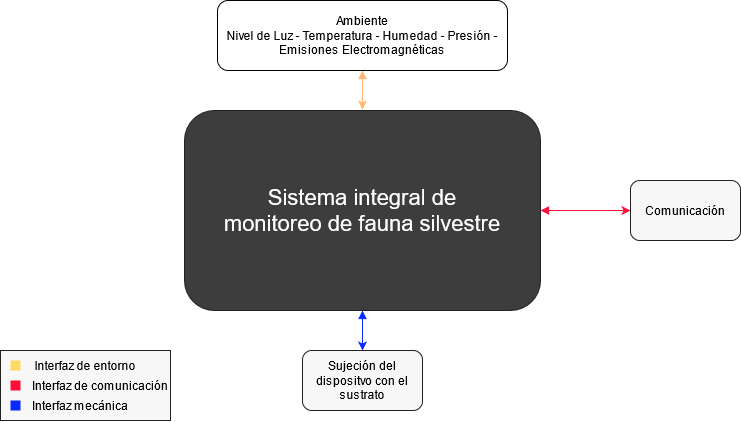
\includegraphics[width=\linewidth]{ImagenesDefinicion/func}
	\label{fig:diagrama_func_interfaces}
	\caption{Diagrama Funcional de Interfaces.}
\end{figure}

\subsection{Especificaciones de Diseño}
\subsubsection{Especificaciones Funcionales}
% Please add the following required packages to your document preamble:
% \usepackage{multirow}
\begin{table}[H]
\centering
\begin{tabular}{|c|c|}
\hline
\multicolumn{2}{|c|}{\textbf{Leyenda para especificaciones}}    \\ \hline
\textbf{Aplicabilidad}             & \textbf{Validación}        \\ \hline
\multirow{2}{*}{P: Prototipo}      & I: Inspección Visual       \\ \cline{2-2} 
                                   & D: Documentación de Diseño \\ \hline
\multirow{2}{*}{F: Producto Final} & S: Simulación              \\ \cline{2-2} 
                                   & T: Test                    \\ \hline
\end{tabular}
\end{table}
\note{Tabla Especificaciones Funcionales}

\note{Tabla 3.5: Especificaciones de Interfaz VOU}
\note{Tabla 3.6: Especificaciones de Interfaz MEC}
\note{Tabla 3.7: Especificaciones de Performance}
\note{Tabla 3.8: Especificaciones de Operación}
\note{Tabla 3.9: Especificaciones de Almacenamiento y Transporte}
\note{Tabla 3.11: Especificaciones Dimensionales y de Peso}
\note{Tabla 3.12: Especificaciones de costos}
\note{Tabla 3.13: Especificaciones de Confiabilidad}
\note{Tabla 3.14: Especificaciones de Disponibilidad}
\note{Tabla 3.15: Especificaciones de Mantenibilidad}
\note{Tabla 3.16: Especificaciones de Seguridad}


\end{document}